\chapter{Systemaufbau und Umsetzung}

\section{Technikstand Fahrrad \(Bellgardt, Menzel\)}
Der Fahrradaufbau dient zur Erfassung von Kräften am Fahrradlenker, indem mechanische Größen in elektrische Signale umgewandelt werden. Dazu werden Dehnungsmessstreifen (DMS) verwendet, die auf relevante Bauteile aufgeklebt werden, um dort auftretende Verformungen zu erfassen. In einer Messbox befindet sich die Messtechnik. Diese zeichnet über die Zeit dann die Belastung auf. Insgesamt befinden sich an dem Lenker 8 DMS. Auf jeder Lenkerseite gibt es jeweils zwei DMS welche als Halbbrücke geschaltet, die Kräfte in horizontaler oder vertikaler Richtung messen. 
Abbildungen \ref{fig:fab3} und \ref{fig:fab4} zeigen den alter Aufbau des Fahrrads.
Um den alten Versuchsaufbau bei Bedarf wieder herstellen zu können musste dieser genau dokumentiert werden.
Dies geschah durch das Beschriften der in der Lenkerbox befindlichen Kabel, siehe \todo{Anhang}


An dem bisherigen Aufbau wurden folgende Optimierungsmöglichkeiten erkannt:
\begin{itemize}
    \item Bisheriger Aufbau am Fahrrad kabelgebunden (USB-Kabel zu PC)
    \item Keine Zugentlastung an der Lenkerbox
    \item Nicht spritzwassergeschützt
    \item Zwischenplatine benötigt
    \item Kontaktierung durch Verschraubung
\end{itemize}

\begin{figure}[h]
    \begin{center}
        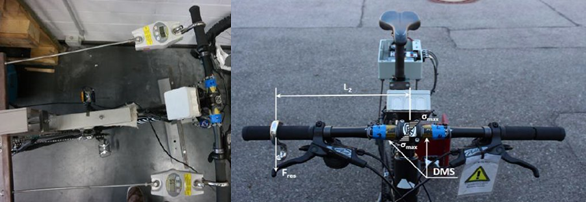
\includegraphics[width=1.0\textwidth, keepaspectratio]{fab3.png}
        \caption[Alter Aufbau des Fahrrads, Lenker (Abbildungsverzeichnis)]{Alter Aufbau des Fahrrads, Lenker
        \footcite{Rechter Teil des Bildes: Praktikum Schwingbruchgefaehrdete Bauteile sicher dimensionieren und betreiben
        }
        }
        \label{fig:fab3}
    \end{center}
\end{figure}


\begin{figure}[h]
    \begin{center}
        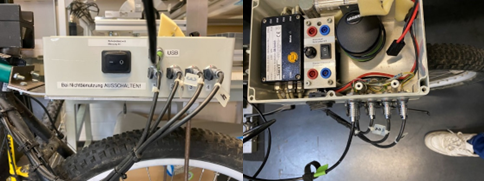
\includegraphics[width=1.0\textwidth, keepaspectratio]{fab4.png}
        \caption[Alter Aufbau des Fahrrads, Messbox (Abbildungsverzeichnis)]{Alter Aufbau des Fahrrads, Messbox}
        %\footcite{Rechter Teil des Bildes: Praktikum Schwingbruchgefaehrdete Bauteile sicher dimensionieren und betreiben
        %}
        
        \label{fig:fab4}
    \end{center}
\end{figure}



\section{Wahl der Komponenten \(Nerb, Ulit\)}


\section{Einbau des V\-Link 200 in ein spritzwassergesch\"utztes Geh\"ause \(Nerb, Ulit\)}
\section{Entwurf der Schaltung und Platine}




\subsection{Umschalter f\"ur Halb\- und Vollbr\"uecke \(Nerb, Ulit\)}
\subsection{Vollbr\"uckenschaltung f\"ur zwei DMS \(Nerb, Ulit\)}

\newpage{}
\subsection{Platinendesign Fahrrad \(Bellgardt, Menzel\)}
Zu Beginn sind wir davon ausgegangen, dass die DMS direkt mit der neuen Messtechnik verbunden werden können, siehe Abbildung \ref{fig:fab5}.
\begin{figure}[h]
    \begin{center}
        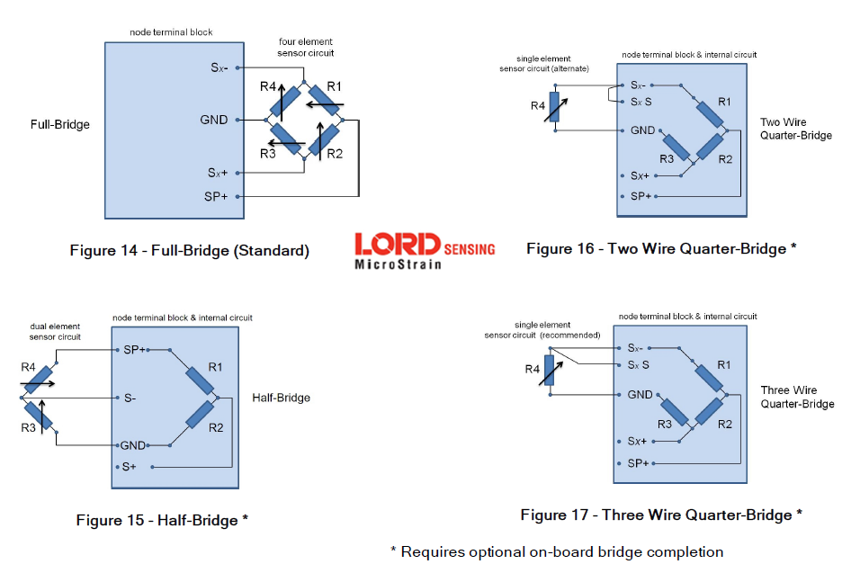
\includegraphics[width=0.9\textwidth, keepaspectratio]{fab5.png}
        \caption[LORD Konfigurationen der Brücken (Abbildungsverzeichnis)]{LORD Konfigurationen der Brücken}
        \footcite{VLInkManual
        }
        
        \label{fig:fab5}
    \end{center}
\end{figure}

Da dies nicht möglich ist, haben wir als Lösung eine Zwischenplatine konstruiert, welche die DMS mit zwei Widerständen zur Halbbrücke ergänzt, siehe Abbildung \ref{fig:fab6}.

\begin{figure}[h]
    \begin{center}
        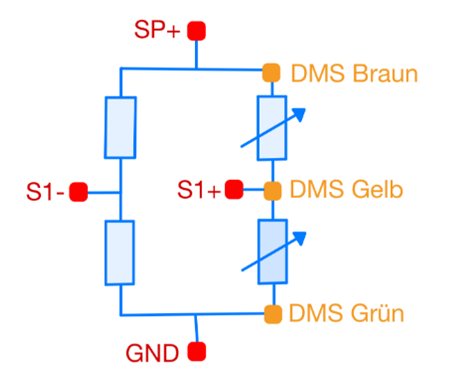
\includegraphics[width=0.4\textwidth, keepaspectratio]{fab6.png}
        \caption[Schaltplan Protoyp Platine (Abbildungsverzeichnis)]{Schaltplan Protoyp Platine}
        %\footcite{VLInkManual
        %}
        
        \label{fig:fab6}
    \end{center}
\end{figure}

Für die Messtechnik sieht dies nun aus wie eine Vollbrücke. Um uns das Wirkungsprinzip und die Funktionsfähigkeit zu verdeutlichen, wurde die Schaltung für den Biegebalken konstruiert.
Der Mittelabgriff des Biegebalkens ist dabei die gelbe Ader. Die Versorgungsapannung von 4,096 V wird durch die Messtechnik vorgegeben und liegt zwischen den Kontakten SP+ und GND an. Der Brückenausgang wird zwischen S1- und S1+ gemessen. Hierüber wird die Belastung der Brücke durch Dehnung der DMS in eine Spannung zwischen S1- und S1+ dargestellt
\subsubsection{Der erste Prototyp}
Basierend auf dem ersten Schaltungsplan wurde dann eine Prototyp-Platine erstellt. Die Platine basiert auf einer Lochplatine. Die verwendeten Widerstände sind 120 Ohm-Metallschichtwiderstände mit einer Abweichung von 1 \%. Der Prototyp wurde am Biegebalken getestet.
\begin{figure}[h]
    \begin{center}
        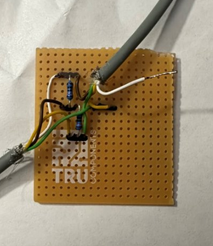
\includegraphics[width=0.4\textwidth, keepaspectratio]{fab7.png}
        \caption[Prototyp Platine mit der Ergänzung der DMS zur Halbbrücke (Abbildungsverzeichnis)]{Prototyp Platine mit der Ergänzung der DMS zur Halbbrücke}
        %\footcite{VLInkManual
        %}
        
        \label{fig:fab7}
    \end{center}
\end{figure}

\subsubsection{Platinenplanung der Lenkerbox}
\todo{fabian reihenfolge erklaerung kicad sinnvoll}
Der Alte Aufbau hat einige Eigenschaften, die durch den neuen Aufbau verbessert wurden. So wurde der alte Aufbau auf einer Lochplatine realisiert.
Zudem wurde die Verbindung der Platine mit Schraubklemmen gelöst. Der Aufbau ist nicht spritzwassergeschützt und die verwendeten Leitungen sind nicht geschirmt.
Die alte Lenkerbox besitzt zudem keine Zugentlastung der Leitungen der DMS Streifen. Es gibt auch keine Zugentlastung der Leitungen zur Messtechnik. 
\begin{figure}[h]
    \begin{center}
        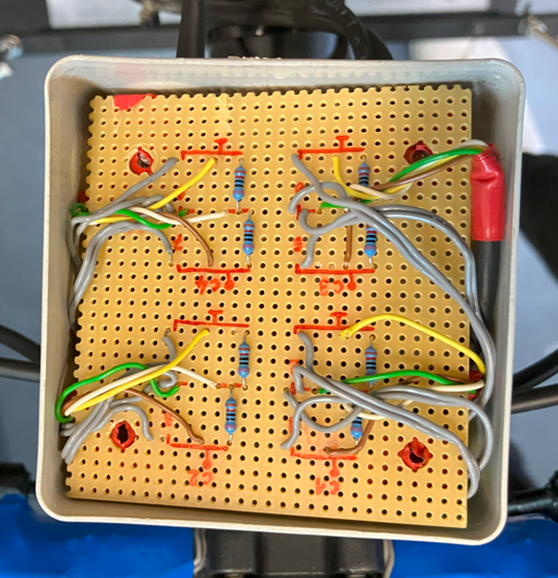
\includegraphics[width=0.3\textwidth, keepaspectratio]{fab8.png}
        \caption[Alte Platine in der alten Lenkerbox (Abbildungsverzeichnis)]{Alte Platine in der alten Lenkerbox}
        %\footcite{VLInkManual
        %}
        
        \label{fig:fab8}
    \end{center}
\end{figure}

Viele der angemerkten Punkte konnten verbessert werden. Hierzu wurde zunächst der Schaltplan in der Software KiCad\footcite{www.kicad.org} eingepflegt.
\todo{fabian reihenfolge erklaerung kicad sinnvoll}

KiCAD ist ein freies Tool, mit welchem man Platinen planen kann. Nach dem erfolgreichen Test der Prototyp Platine an dem Biegbalken wurde die Schaltung hochskaliert. Der Hauptunterschied im Anschluss der DMS des Biegebalkens und denen des Fahrrads besteht darin, dass der Mittelabgriff am Fahrrad durch die weißen DMS bereitgestellt wird.
\begin{figure}[h]
    \begin{center}
        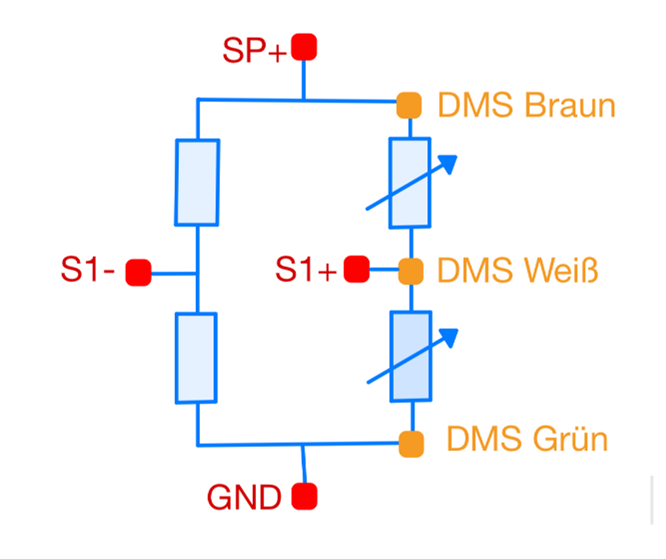
\includegraphics[width=0.4\textwidth, keepaspectratio]{fab9.png}
        \caption[Schaltungsplan Fahrrad (Abbildungsverzeichnis)]{Schaltungsplan Fahrrad}
        %\footcite{VLInkManual
        %}
        
        \label{fig:fab9}
    \end{center}
\end{figure}

\subsubsection{Planung der Schaltung mit KiCAD}
In der Software KiCAD\footcite{www.kicad.org} wurde zunächst ein Schaltplan erstellt, siehe \ref{fig:fab11}.
\begin{figure}[h]
    \begin{center}
        
\includegraphics[width=0.2\textwidth, keepaspectratio]{fab10.png}
        \caption[KiCad Software Logo (Abbildungsverzeichnis)]{KiCad Software Logo}
        \footcite{www.kicad.org}
        \label{fig:fab10}
    \end{center}
\end{figure}


Dieser stellt 4 Halbbrücken dar.
Auf der Platine werden pro Halbbrücke je zwei Widerstände angebracht. Die befinden sich in Form ihrer Kontakte auf der Platine.
Basierend auf dem Schaltplan (siehe Anhang: )\todo{Daniel: Verweis zur Schaltplan PDF in Anhang packen} wurde dann die Platine zunächst entsprechend Ihrer Abmessungen für das Gehäuse simuliert (siehe \ref{fig:fab12}) und anschließend gedruckt. Die fertige Platine ist in der Abbildung \ref{fig:fab13}zu sehen. Sie besitzt die Maße des Gehäuses. Zudem verfügt die Platine über 4 zusätzliche Bohrungen, um sie besser im Gehäuse befestigen zu können. 
\begin{figure}[h]
    \begin{center}
        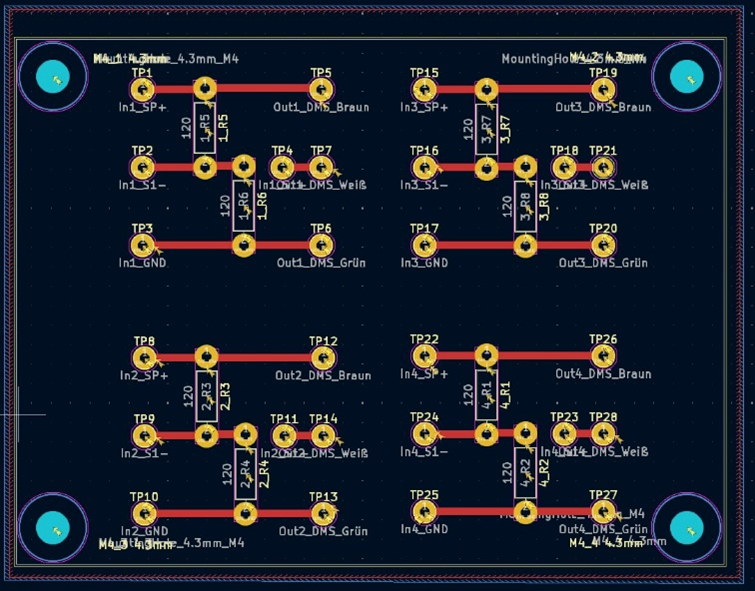
\includegraphics[width=0.4\textwidth, keepaspectratio]{fab11.png}
        \caption[Planung Lenkerplatine (Abbildungsverzeichnis)]{Planung Lenkerplatine}
        %\footcite{www.kicad.org}
        \label{fig:fab11}
    \end{center}
\end{figure}

\begin{figure}[h]
    \begin{center}
        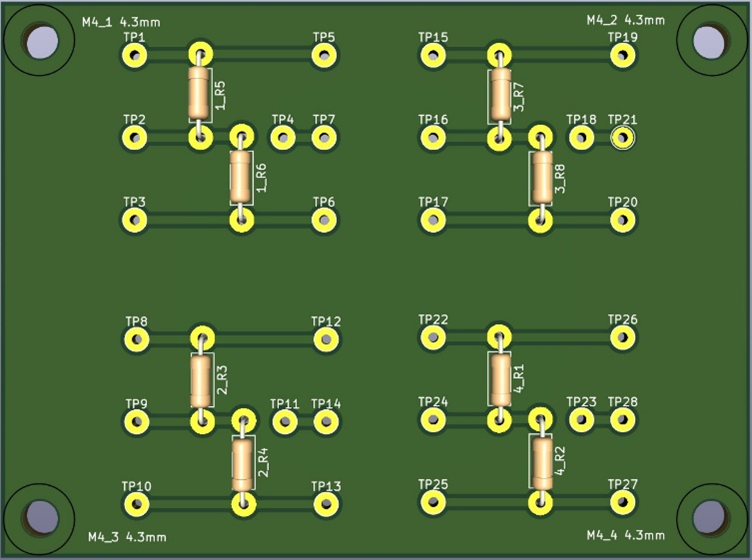
\includegraphics[width=0.4\textwidth, keepaspectratio]{fab12.png}
        \caption[Simulation der Lenkerplatine (Abbildungsverzeichnis)]{Simulation der Lenkerplatine}
        %\footcite{www.kicad.org}
        \label{fig:fab12}
    \end{center}
\end{figure}

\begin{figure}[h]
    \begin{center}
        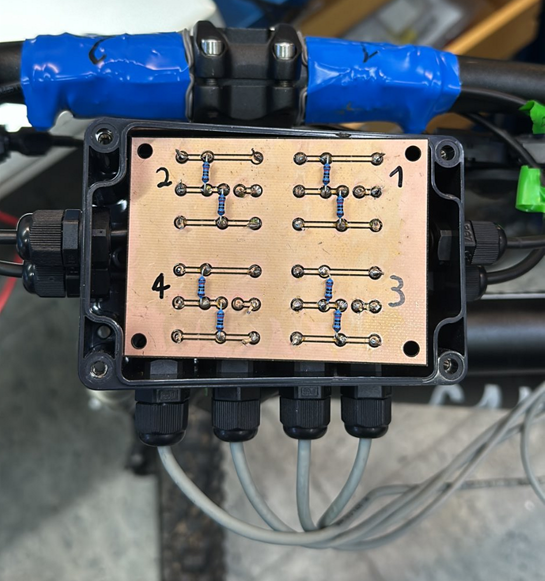
\includegraphics[width=0.4\textwidth, keepaspectratio]{fab13.png}
        \caption[Fertig installierte Lenkerplatine (Abbildungsverzeichnis)]{Fertig installierte Lenkerplatine}
        %\footcite{www.kicad.org}
        \label{fig:fab13}
    \end{center}
\end{figure}





\newpage{}

\subsection{Platinendesign Suit \(Nerb, Ulit\)}
\section{Herstellung der Acrylplatte f\"ur die Geh\"auseintegration \(Nerb, Ulit\)}
\section{Montage und Verbindung der DMS \(Nerb, Ulit\)}
